\documentclass{article}

\usepackage[most]{tcolorbox}
\usepackage{physics}
\usepackage{graphicx}
\usepackage{float}
\usepackage{amsmath}
\usepackage{amssymb}


\usepackage[utf8]{inputenc}
\usepackage[a4paper, margin=1in]{geometry} % Controla los márgenes
\usepackage{titling}

\title{clase 15 }
\author{Manuel Garcia.}
\date{\today}

\renewcommand{\maketitlehooka}{%
  \centering
  \vspace*{0.05cm} % Espacio vertical antes del título
}

\renewcommand{\maketitlehookd}{%
  \vspace*{2cm} % Espacio vertical después de la fecha
}

\newcommand{\caja}[3]{%
  \begin{tcolorbox}[colback=#1!5!white,colframe=#1!25!black,title=#2]
    #3
  \end{tcolorbox}%
}

\begin{document}
\maketitle

\section{Tensores totalmente antisimétricos}
$ \omega_r  $ tensores de tipo $ (0,r) \rightarrow \Omega _p^r(M) $

Vamos a definir las permutacion y la accion de una permutacion sobre un tensor de tipo $ (0,r) $.
\begin{gather*}
  p\omega (v_1,...,v_r) = \omega(v _{p(1)} , ..., v _{p(r)} )\\
  p \in S_r \rightarrow \text{Grupo simetrico de orden }r \\
  \textbf{Ejemplo: }\\
  \omega(v_1,v_2,v_3) \qquad \qquad S_3 = \{ \underset{p1}{(1,2,3)}, \underset{p_2 }{(1,3,2)}, \underset{p_3}{(2,1,3 )}, \underset{p_4 }{(2,3,1 )}, \underset{p_5 }{(3,1,2)}, \underset{p_6 }{(3,2,1 )} \} \\
  p_4\omega(v_2,v_2,v_3) = \omega (v_2,v_2,v_1 )
\end{gather*}
Con la forma: $ \{e_\mu \} = \{\frac{\partial  }{\partial x ^ {\mu }} \}$
\begin{align*}
  \omega _{\mu_1,...,\mu_r } &= \omega(e_{\mu_1},...,e _{\mu_r } )\\
  p(\omega_{\mu_1,..., \mu_r }) &= \omega(e _{p(\mu_1)} , ..., e _{p(\mu_r )} )\\
  &= \omega _{p(\mu_1) \dots p(\mu_r)}
\end{align*}

Vamos a trabajar con el siguiente simetrizador: 
\caja{red}{Simetrizador}{
  \begin{gather*}
    S\omega = \frac{1}{r!} \displaystyle\sum_{p\in S_r }^{} p\omega 
  \end{gather*}
}
\textbf{Ejemplo }
\begin{gather*}
  \omega \in J ^ {0 } _{2, p } (M) \qquad \qquad S_2 = \{(1,2),(2,1)\}\\
  S\omega = \frac{1}{2! } [\omega(v_1,v_2) + \omega(v_2,v_1)]\\
\end{gather*}

El antisimetrizador: 
\caja{red}{Antisimetrizado}{
  \begin{gather*}
    A\omega = \frac{1}{r! } \displaystyle\sum_{p\in S_r }^{} sgn(p) p\omega \qquad \qquad sgn(p) = \begin{cases}
        +1 & \text{par }\\
        -1 & \text{impar }
    \end{cases}
  \end{gather*}
}

Ahora vamos a tomar una \textit{r-forma } o tensor tipo $ (0,r ) $ completamente antisimétrica. 
$ T _{\sigma(\mu_1,\dots, \mu_r )} = sgn(\sigma) T _{\mu_1,\dots, \mu_r )}  $
\textbf{Ejemplo: } para $ T _{\mu_1,\mu_2,\mu_3}  $
\begin{gather*}
  T _{\mu_3,\mu_2,\mu_1} = T_{\mu_1,\mu_2,\mu_3}\qquad\qquad T_{\mu_1,\mu_3,\mu_2}  = - T_{\mu_1,\mu_2,\mu_3}\\
  r=3 \qquad dx ^ {\mu_1 }\land dx ^ {\mu_2 } \land dx ^ {\mu_3 } = dx ^ {\mu_1 }\otimes dx ^ {\mu_2 } \otimes dx ^ {\mu_3 }
\end{gather*}
En general: $\qquad dx ^ {\mu_1 }\land \dots \land dx ^ {\mu_r } = \displaystyle\sum_{\sigma \in S_r }^{} sgn(\sigma) e ^ {\sigma(\mu_1 )} \otimes \dots \otimes e ^ {\sigma(\mu_r )}$


Qué sucede si se repite $ \mu_1 = \mu_2 = \mu $
\begin{gather*}
  (dx ^ {\mu} \land dx ^ {\mu })\land dx ^ {\mu_3 }\\
  \text{Tenemos que } \quad dx ^ {\mu} \land dx ^ {\mu } = - dx ^ {\mu } \land dx ^ {\mu } \\
  2dx ^ {\mu}\land dx ^ {\mu } = 0 
\end{gather*}

\caja{black}{propiedades producto $ \land  $}{
  \begin{itemize}
    \item $ dx ^ {\mu}\land dx ^ {\mu } = 0 $
    \item $ dx ^ {\mu_1 } \land \dots\land dx ^ {\mu_r } = sgn(\sigma) dx ^ {\sigma(\mu_1)} \land \dots \land dx ^ {\sigma(\mu_r )} $
    \item $ dx ^ {\mu_1 } \land \dots\land dx ^ {\mu_r } $ es lineal en cada $ dx ^ {\mu_1 } $.
  \end{itemize}
}

\textbf{Vamos a escribir el simetrico con [] y el antisimetrico con ()}

\hfill 

\hfill 

En el punto $ p\in M  $ denotados por $ \Omega _p^r(M) $ al espacio de todas las r formas. Las bases de este espacio son los elementos 
\begin{gather*}
  dx ^ {\mu_1 }\land \dots\land dx ^ {\mu_r }\\
  T = \frac{1}{r! }T _{\mu_1, \dots, \mu_k} dx ^ {\mu_1 }\land \dots\land dx ^ {\mu_k }
\end{gather*}

\begin{figure}[H]
  \begin{center}
    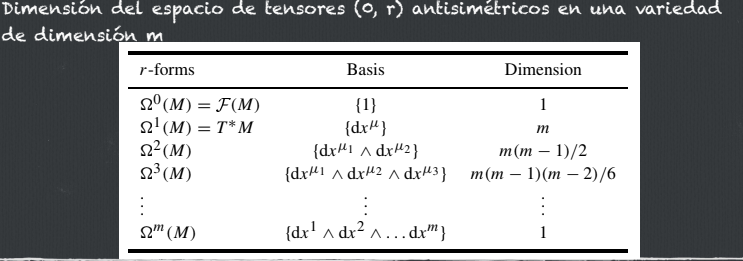
\includegraphics[width=0.95\textwidth]{dim_tensores_antisimetricos.png}
  \end{center}
\end{figure}

\textbf{Antisimetricos: } numero de componentes independientes: 
\begin{gather*}
  \binom{m}{r} = \frac{m!}{r!(m - r)!}
\end{gather*}

\textbf{Simetricas:} 
\begin{gather*}
  \binom{m+r-1 }{r} = \frac{(m+r-1)! }{r!(m-1)!}
\end{gather*}

\textbf{Ejemplo} 
\begin{gather*}
  T _{\mu v } = \frac{1}{2} (T _{\mu v }  + T _{v \mu }  + T _{\mu v }  - T _{v \mu } )\\
  T _{\mu v } = \underset{simetrico }{T _{(\mu v )} }+ \underset{antisimetrico }{ T _{[\mu v ]}}\\
  m ^2 = \frac{(m+1)! }{2! (m+1)! } + \frac{m! }{2!(m-2)! } = m^2
\end{gather*}
\begin{gather*}
  T _{\mu v \alpha } \overset{?}{=} T _{(\mu v \alpha) } + T _{[\mu v \alpha ]} \\
  m ^3 \overset{?}{=} \frac{(m + 2 )! }{3! (m-1)! } + \frac{m! }{3! (m-3)! } \\
  m^3 = \frac{m }{3 }(m^2 + 2 )
\end{gather*}

\textbf{Propiedad: } $ dim(\Omega _p^r (M)) = dim(\Omega_p^{m-r}(M)) $ son isomorfos.

\hfill 

\hfill 

\hfill 

\begin{gather*}
  \omega \land \xi (v_1,...v _{q + r } ) \in \Omega _p ^ {q + r }(M) \\
  \equiv \frac{1}{r!q! } \displaystyle\sum_{r\in S _{q + r } }^{}sgn(\sigma ) \omega (V _{\sigma(1) } \dots V _{\sigma(q)} ) \times \xi (V _{\sigma{(q + 1 )}} , \dots, V _{\sigma(q+r)} )\\
  \omega\land \xi = (-1)^ {qr } \xi \land \omega\\
  \xi \land \omega = \frac{1}{r! q! } \displaystyle\sum_{\sigma\in S _{q + r } }^{} sgn(\sigma) \xi (V _{\sigma(1) } , \dots, V _{\sigma(r)} ) \omega (V _{\sigma(r+1)} , \dots, V _{\sigma(r + q )} )
\end{gather*}

\subsection{Derivada exterior }
El producto exterior nos va a aumentar el grado de la forma en una dimension 
\caja{red}{Derivada exterior }{
  \begin{gather*}
    d \omega  = \frac{1}{r! } \partial _{[_\alpha\omega _{\mu_1,\dots, \mu_r } ]}dx ^ {\alpha } \land dx ^ {\mu_1 } \land \dots\land dx ^ {\mu_r }
  \end{gather*}
}
\textbf{Ejemplo: } Todas las posibles r-formas en 3 dimensiones: 
\begin{gather*}
  \omega_0 = \omega_0 (x,y,z) \\
  \omega_1 = \omega_x dx + \omega_y dy + \omega_z dz\\
  \omega_2 = \omega _{xy } dx \land dy + \omega _{yz } dy \land dz + \omega _{zx } dz \land dx \\
  \omega_3 = \omega _{xyz } dx \land dy \land dz 
\end{gather*}

Y sus derivadas exteriores: 
\begin{gather*}
  d \omega_0 = \frac{\partial f  }{\partial x } dx + \frac{\partial f  }{\partial  y }dy  + \frac{\partial f  }{\partial  z } dz \\
  ...
\end{gather*}

\end{document}
